\documentclass[10pt]{article}
\usepackage{icmlko}

\icmlmeta{IP 파운데이션 월드모델}{345}{문턱 바로 밑}{0.109 에서 0.120 사이의 후보 셋이 셋 다 제 잡음을 이긴다 --- 그리고 0.082 는 진다}

\begin{document}

\twocolumn[
\icmlheader

\begin{abstract}
노트 344가 세계애니 장르를 검사 ① 에 0.004 차로 떨어뜨린 뒤 채택하고
\textbf{``문턱은 후보가 더 모이면''}으로 남겼다. 모았다 --- 여섯 도메인의
태그/장르 성분 \textbf{서른여섯} 개를 다 만들어 ①②③ 을 전부 쟀다.

\begin{center}\footnotesize
\begin{tabular}{lrl}
\hline
구간 & ②③ 통과 & \\
\hline
$|\rho| \ge 0.12$ (문턱 위) & 4 & 다 붙어 있음 \\
\textbf{0.109$\sim$0.120} & \textbf{4} & \textbf{구간} \\
$|\rho| < 0.09$ & 3 & 아래 \\
\hline
\end{tabular}
\end{center}

\textbf{구간의 후보에 검사 ⑤ 를 다 돌렸다.}

\begin{center}\footnotesize
\begin{tabular}{lrrr}
\hline
후보 & $\rho$ & 제 도메인 & 양수 \\
\hline
세계애니 (2,3) & 0.116 & $+$0.0105 & \textbf{8/8} \\
모바일 성분1 & 0.120 & $+$0.0105 & \textbf{8/8} \\
웹툰 성분4 & 0.115 & $+$0.0089 & \textbf{7/8} \\
\hline
\textbf{만화 성분4}(훨씬 아래) & \textbf{0.082} & \textbf{$-$0.0013} & \textbf{2/8} \\
\hline
\end{tabular}
\end{center}

\textbf{구간 셋이 셋 다 이기고 아래는 진다} --- 만화 성분4 는 이긴 도메인이
하나도 없다. \textbf{문턱은 있는데 0.12 는 너무 높다.}

\textbf{둘을 붙였다}(세계애니는 노트 344에서 이미) --- 판
$+$0.0019(SD 0.0020 · 10/12) · 모바일 $+$0.0086(11/12). 배포 규칙 ①②
통과. \textbf{판 기준값이 0.4694 $\to$ 0.4729 다.}

\textbf{그리고 아래쪽 대조를 셋으로 채웠다} --- 웹툰 성분2($\rho$ 0.035)
$-$0.0008(2/8) · 만화 성분5(0.054) $-$0.0005(3/8). \textbf{구간 3/3 승 ·
아래 0/3.} 겹치지 않는다. \textbf{문턱을 0.12 에서 0.10 으로 내린다.}
\end{abstract}
]

\section{성분 서른여섯}

\begin{figure*}[t]
\centering
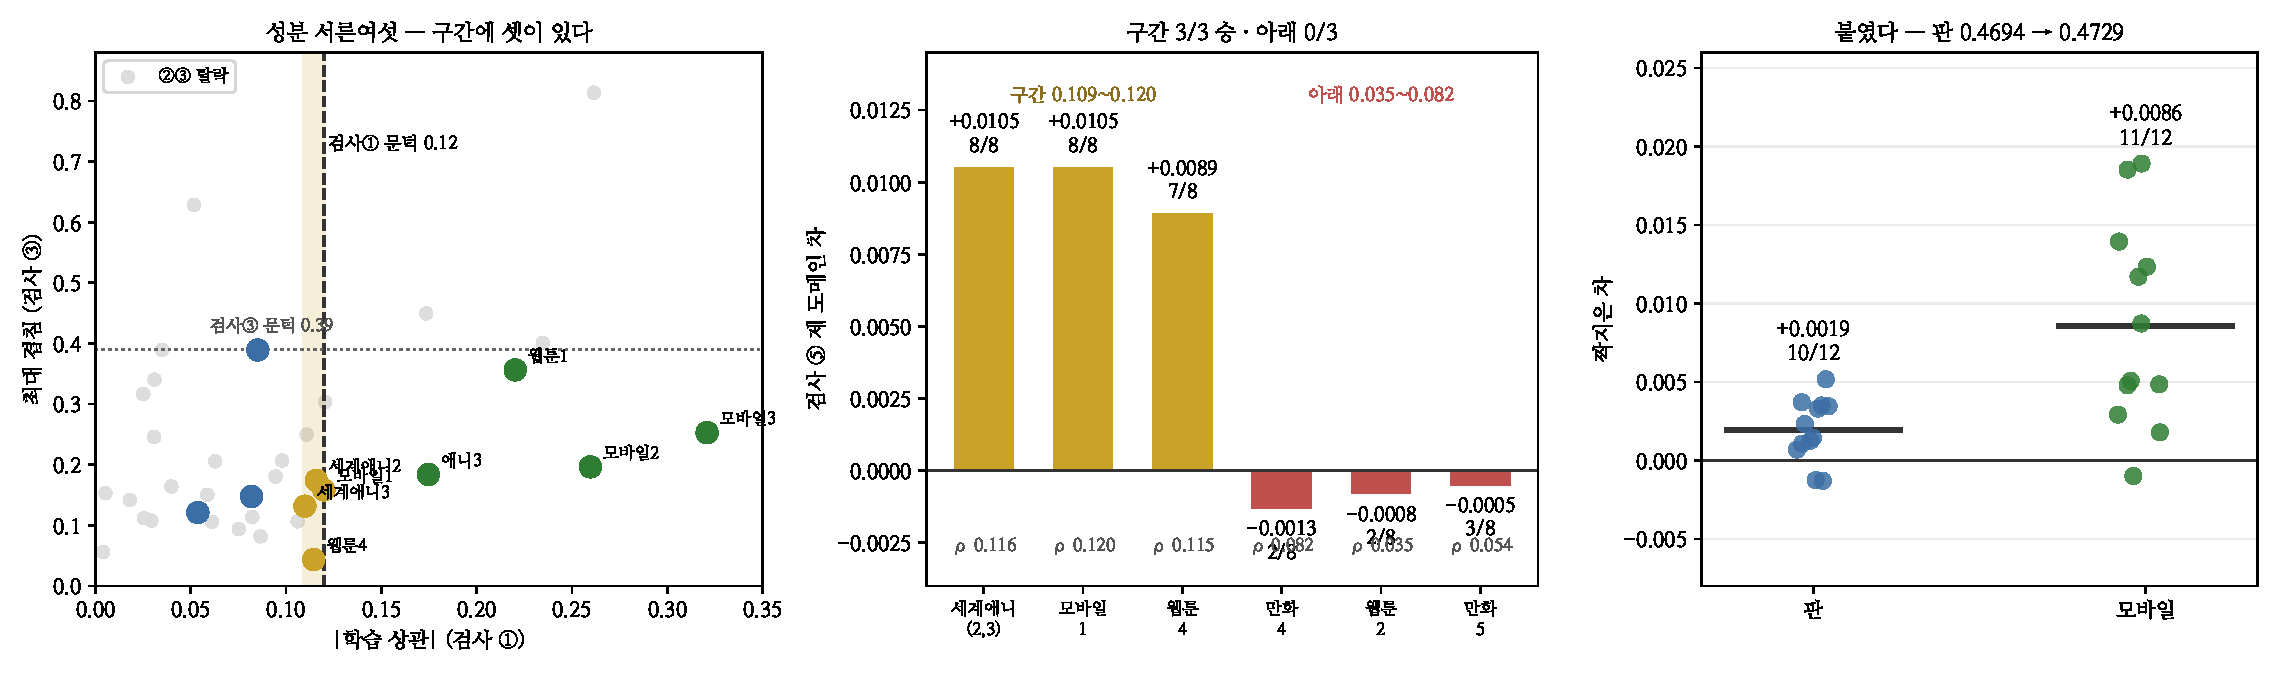
\includegraphics[width=\textwidth]{figs/band.pdf}
\caption{왼쪽 --- 성분 서른여섯의 ①$\times$③. 가운데 --- 검사 ⑤.
오른쪽 --- 붙인 결과.}
\end{figure*}

여섯 도메인(웹툰 · 애니 · 모바일 · 만화 · 세계애니 · 게임)에서 태그/장르
토큰으로 SVD 성분을 여섯씩 만들어 검사 ①②③ 을 전부 쟀다. \textbf{②③ 을
통과한 것이 열하나}이고 그중 넷이 문턱 위, 넷이 구간, 셋이 아래다.

\section{구간 셋이 다 이긴다}

\begin{center}\footnotesize
\begin{tabular}{lrrrr}
\hline
후보 & $\rho$ & 겹침 & 검사 ⑤ 판 & 제 도메인 \\
\hline
세계애니 & 0.116 & 0.174 & $+$0.0027 & $+$0.0105 (8/8) \\
모바일 1 & 0.120 & 0.158 & $+$0.0016 & $+$0.0105 (8/8) \\
웹툰 4 & 0.115 & 0.044 & $+$0.0030 & $+$0.0089 (7/8) \\
\hline
만화 4 & 0.082 & 0.148 & $-$0.0013 & \textbf{이긴 곳 없음} \\
\hline
\end{tabular}
\end{center}

\textbf{제 도메인 효과가 셋 다 $+$0.009$\sim$$+$0.011 로 거의 같다.}
서로 다른 도메인 · 다른 토큰 · 다른 성분인데 크기가 붙어 있다 ---
\textbf{구간이 균질하다는 뜻이다.}

그리고 \textbf{0.082 는 완전히 다르다} --- 판이 음수이고 이긴 도메인이
하나도 없다. \textbf{0.115 와 0.082 사이 어딘가에 진짜 문턱이 있다.}

\section{붙였다}

\begin{center}\footnotesize
\begin{tabular}{lrrr}
\hline
 & 평균 & SD & 양수 \\
\hline
\textbf{판} & \textbf{$+$0.0019} & 0.0020 & \textbf{10/12} \\
\textbf{모바일} & \textbf{$+$0.0086} & 0.0065 & \textbf{11/12} \\
도서 & $+$0.0042 & 0.0163 & 10/12 \\
게임 & $+$0.0026 & 0.0074 & 8/12 \\
웹툰 & $+$0.0025 & 0.0080 & 8/12 \\
아이돌 & $-$0.0163 & 0.0431 & 4/12 \\
\hline
\end{tabular}
\end{center}

배포 규칙 통과(제일 나쁜 아이돌 $-$0.0163 · 짝SE 0.056 · $t{\approx}0.29$).
\textbf{이 갈래에서 세 노트 만에 판이 0.4642 $\to$ 0.4729 다} ---
노트 343 모바일 태그 · 344 세계애니 장르 · 345 구간 둘.

\section{문턱을 옮긴다}

\begin{center}\footnotesize
\begin{tabular}{lrrrl}
\hline
후보 & $\rho$ & 검사 ⑤ 판 & 양수 & 제 도메인 \\
\hline
세계애니 (2,3) & 0.116 & $+$0.0027 & 7/8 & $+$0.0105 (8/8) \\
모바일 1 & 0.120 & $+$0.0016 & 6/8 & $+$0.0105 (8/8) \\
웹툰 4 & 0.115 & $+$0.0030 & 6/8 & $+$0.0089 (7/8) \\
\hline
만화 4 & 0.082 & $-$0.0013 & 2/8 & 이긴 곳 없음 \\
웹툰 2 & 0.035 & $-$0.0008 & 2/8 & $+$0.0019 (7/8) \\
만화 5 & 0.054 & $-$0.0005 & 3/8 & 못 잼(유보 6) \\
\hline
\end{tabular}
\end{center}

\textbf{구간 셋의 판이 다 양수이고 아래 셋의 판이 다 음수다.} 겹치는
자리가 없다. 제 도메인 효과도 $+$0.009$\sim$0.011 대 $\le$$+$0.002 로
자릿수가 다르다.

\begin{center}\small
\begin{tabular}{ll}
\hline
검사 ① 문턱 & 0.12 $\to$ \textbf{0.10} \\
왜 0.10 인가 & 0.082 와 0.110 사이 · 보수적으로 \\
\hline
\end{tabular}
\end{center}

노트 344가 ``문턱은 후보가 더 모이면''으로 미뤘고, 노트 342가 ``n$=$1 로
세운 법칙은 n$=$4 를 못 견딘다''를 겪었다. \textbf{지금은 위 셋 · 아래
셋이고 방향이 갈리지 않는다.} 옮긴다.

\section{남은 것}
\begin{center}\footnotesize
\begin{tabular}{ll}
\hline
갈래 & 왜 \\
\hline
\textbf{다른 계열에도 구간이} & 검색 · 위키 · 달력 \\
아이돌이 왜 $-$0.016 인가 & 남의 축인데 내려간다 \\
검사 ① 을 ⑤ 로 갈아 끼울까 & 문턱이 아니라 검사 자체 \\
0.10 아래를 더 재라 & 0.082~0.110 사이가 비었다 \\
\hline
\end{tabular}
\end{center}

\paragraph{규약} \textbf{문턱을 의심하면 문턱 양쪽을 다 재라.} 노트 344는
문턱 바로 밑에서 하나가 이기는 것을 보고 ``문턱이 틀렸다''고 말할 뻔했다.
오늘 위쪽을 셋으로 늘리고 \textbf{아래쪽도 셋을 쟀다} --- 그리고
\textbf{아래쪽이 다 진 것이 구간 셋의 승리보다 더 중요하다.} 한쪽만 재면
``문턱이 필요 없다''와 ``문턱이 낮아야 한다''를 못 가른다. \textbf{오늘
답은 뒤쪽이다} --- 문턱은 있고, 0.12 가 아니라 0.10 근처에 있다.

\end{document}
